\documentclass[a4paper,12pt]{article}
\makeatletter

\usepackage{graphicx}
\usepackage{amsmath}
\usepackage{textcomp}
\usepackage{amsfonts}
\usepackage{amssymb}
\usepackage{epstopdf}
\usepackage{epsfig}
\usepackage[small,it]{caption}
\usepackage{setspace}

\usepackage[style=authoryear,
maxcitenames=2,
maxnames = 2,
firstinits=true,
uniquename=init,
sorting=nty,
url=false,
isbn=false,
eprint=false,
doi=false,
texencoding=utf8,
bibencoding=utf8,
backend=bibtex]{biblatex}

\bibliography{../library.bib}

\begin{document}
\begin{center}
\textbf{Report for the capstone project: predict building abandonment in Detroit}
\end{center}

\paragraph{Methods}
For this project I have mainly used python, in particular using the Ipython notebooks as an interface. For calculation and data structures I have used numpy and pandas. For the machine learning methods I have used the scikit-learn package. For the spatial analysis, distance calculation and addresses checking I used the geopy package. For initial visualisation and data exploration I have used Tableau. For data visualisation in python I have used Folium on python and Basemap.

\paragraph{Building definition}
I build my building list using the incident dataset. In particular we assume every incident to be a building, and we define the building as a rectangle centred on the incident coordinate. The first thing to define is the size of the triangle, we decided to go for 100 m per side. In practice centre, bottom and top left and right corners of the building are stored. This makes it quite easy to check whether an event is within the building since it doesn't require any distance calculation but only comparisons. I also considered a definition of a building using the incident as a centre of a circle of some radius, $\sim$ 50 m to be consistent with the previous definition. The problem with this kind of definition however is that is makes it complicated to establish if a certain event is within the building as a distance calculation is required. This is a fairly easy task using some geolocation package, however the calculation time doesn't scale up very well and in fact creates problem even with the blight definition we have to make in the following section. For this reason it was abandoned.\\
\\
Once we identified the buildings we checked whether we were considering the same building multiple times checking the distance between the building's centres. Moreover we used geopy to compare the address to the coordinates, in case they didn't match we used the address to get the correct coordinates.\\
\\
\paragraph{Bighted building labelling}
To label building we used the demolition permits dataset, for every demolition permit falling within 100 m from a building we labelled the building as blighted. With this method we came up with a 5927 blighted buildings. Given this set of $\sim$ 6000 blighted building we also randomly select an equal amount of non blighted building for a total of $\sim$ 12000 building dataset, see Fig. \ref{label}.

\begin{figure}
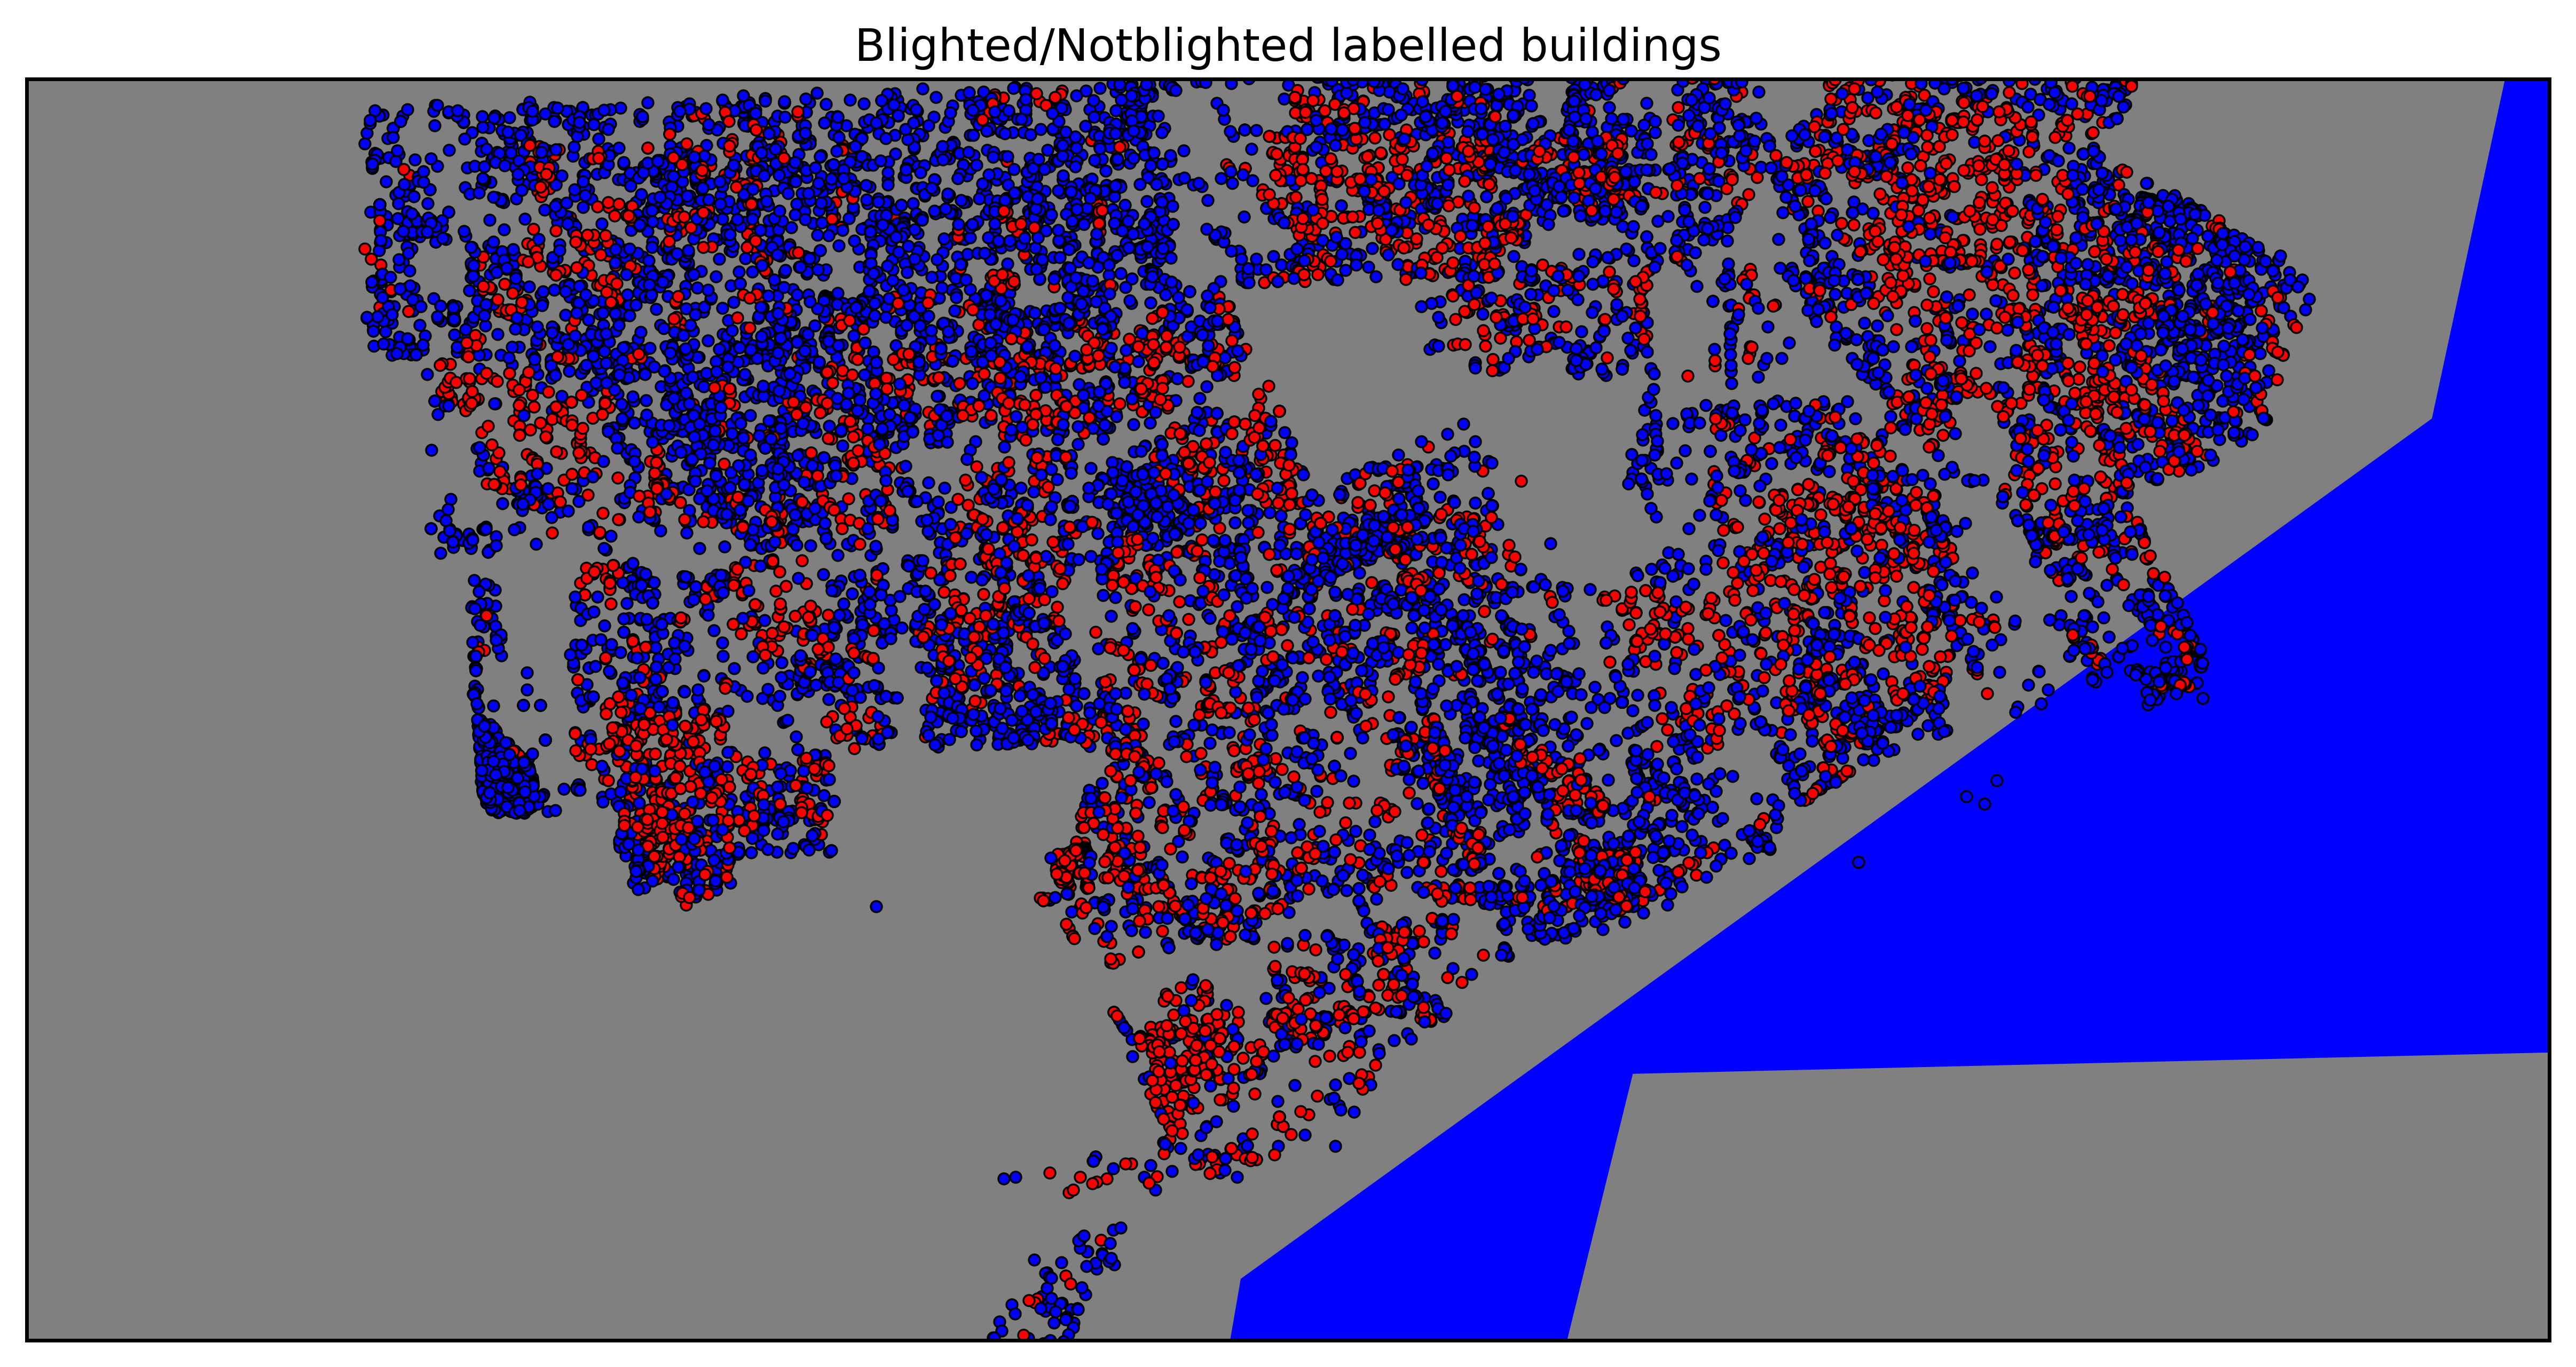
\includegraphics[scale=0.55]{label.png}
\caption{Map of the labelled buildings with blighted in red and non blighted in blue}
\label{label}
\end{figure}

\paragraph{First basic model}
Using the blight violation dataset we calculated a basic feature for each building: the number of blight violations associated to the building. With this feature we trained three model to predict blighted buildings: a logistic regression model, a decision tree model and a random forest model. These three models should theoretically provide similar but different results using different features and will be used in the following  too. This very simple model can't possibly be expected to provide high accuracy but as a first step we are interested in understanding whether we can get a positive results, i.e. an accuracy greater than $\sim 50 \%$. The results are positive giving an accuracy around $\sim 60 \%$ for every model. In particular: 
Logistic Regression 0.602, Decision tree 0.595,
Results for Random Forest 0.595. The results are quite acceptable given the very basic feature considered.

\paragraph{Increasing the accuracy of the model}
Given the large amount of data provided it is possible to consider many feature to add to the model. Personally before setting with a final model I have considered the following,a and developed and tested models with some variations of these features:
\begin{itemize}
\item Expand the blight violation feature, consider blight violations within 100, 200, 500 meters and so on. Blight violations in the neighbourhood could be indicative of a general neighbourhood condition. Consider blight violation costs, with the assumption the higher the cost is the more serious the violation is.
\item Consider the crime dataset. This datasets consists of a crimes committed in Detroit, each crimes is classified in a list of 50 crime types, and has a date time and locations. Possible features to consider for the model are general number of crimes within a certain distance from thee building, presence of not of a certain type of crime within a certain distance from the building, number of a certain type of crime. 
\end{itemize}
As a first try I considered blight violations within a 250 m radius from the building and the cost of blight violations as supplementary features. Unfortunately these features didn't prove to be very useful with basically no increase in the model accuracy. Any combination of the previously  described three features gives an accuracy no higher than $\sim 60 \%$.
\begin{figure}
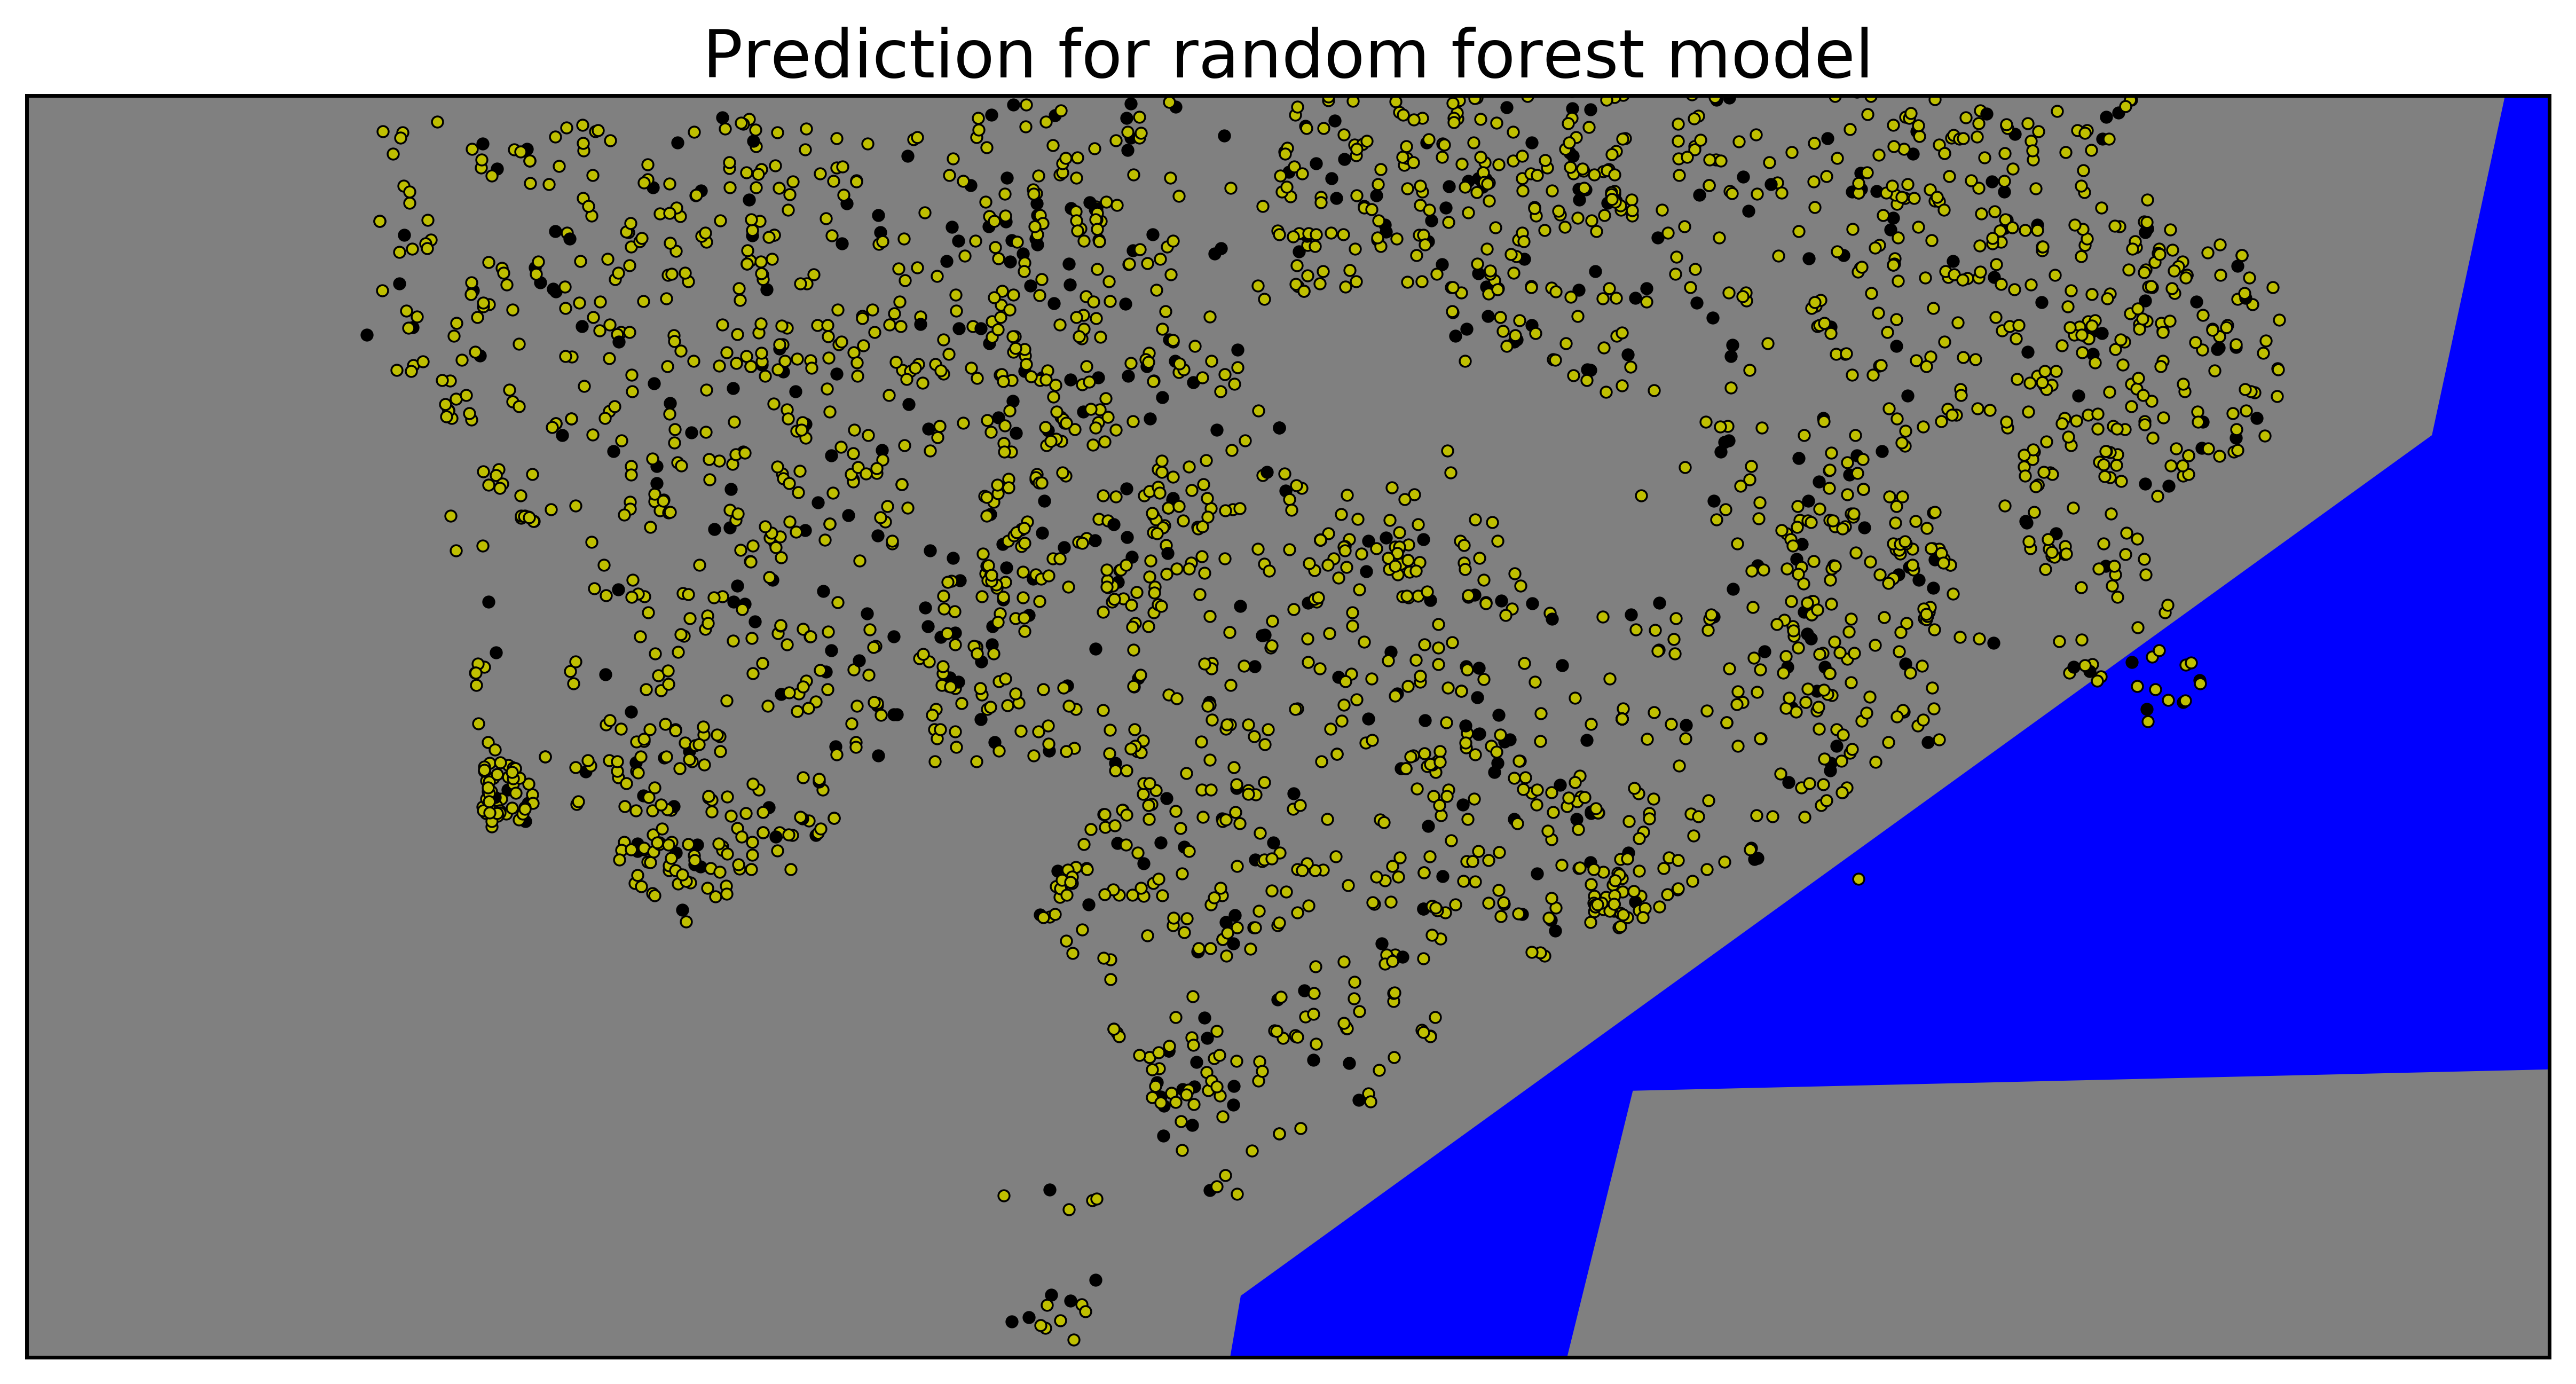
\includegraphics[scale=0.55]{predict.png}
\caption{Map of the random forest predictions with right predictions in yellow and wrong predictions in black}
\label{pred}
\end{figure}
Given the poor results of the previous developed features I used the crime dataset to develop new features. In particular I used a counter for every crime within 500 meters and counter for specific type of crime within 500 meters. I experimented with combinations of the new features and the previously developed features. The best results obtained was using the only the crime-specific 50 features and the random forest model, that gave an accuracy of $78\%$, the decision tree model gave a similar accuracy of $75\%$. Figure \ref{pred} shows the model random forest model predictions.

\paragraph{Further improvements that might be considered}
Many other possible improvements could be implemented in the model. The use of three different models using different labels showed that the most important characteristic to improve model performances is not the specific algorithm used but the layers. Therefore improvements on the model would need to be focused on developing new features. This could be done in various way: an example could be taking into consideration the time of various events considered: crimes, demolition permits, violations.

\end{document}